\section{Assessment of Compatibility with Emission Models} \label{sec:emission}
% ============================================================================
\subsection{Spectral Shape} \label{sec:shape}
Optically-thin synchrotron limits the low-energy index to
$\alpha\le-2/3$ (slow cooling), steepening to $-3/2$ (fast cooling), whereas a
photosphere can be harder; a photospheric preference can be claimed with
confidence only for $\alpha>-0.5$ at high significance \citep{Acuner2020}. We
place the maximum $\alpha$ of each burst against \Ep\ and the synchrotron and
photospheric limiting lines (Figure~\ref{fig:lines}). We find that $74\%$
($74/100$) of bursts reach a peak $\alpha$ above the slow-cooling synchrotron line
($-2/3$) and $64\%$ ($64/100$) enter the photospheric region ($\alpha>-0.5$),
broadly consistent with the hard low-energy indices reported by \citet{Basak2014}
and \citet{Crider1997} and difficult to reconcile with pure fast-cooled
synchrotron.

\begin{figure}[t]
\centering
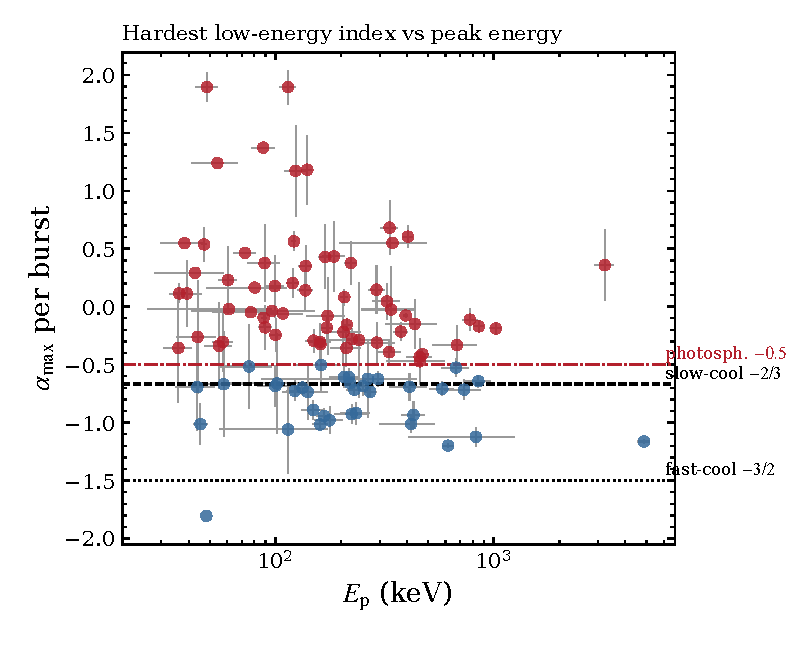
\includegraphics[width=\linewidth]{two_break_figures/fig_lines.pdf}
\caption{Hardest low-energy index per burst, $\alpha_{\rm max}$, vs \Ep, with the
slow- and fast-cooled synchrotron lines ($-2/3$, $-3/2$) and the photospheric
limit ($-0.5$). Red points (64/100) reach the photospheric region in at least one
bin. The few extreme values ($\alpha_{\rm max}\gtrsim1$) arise from weakly
constrained bins and carry correspondingly large uncertainties.}
\label{fig:lines}
\end{figure}

\subsection{Spectral Evolution and Correlations} \label{sec:evol-assess}
The curvature split (Section~\ref{sec:curv}) indicates that most single-pulse
curvature is statistically consistent with an added blackbody, with a minority
decisively requiring a second synchrotron break. The sub-dominant
$F_{\rm BB}/F_{\rm tot}$, the recovery of the $\Ep$--$\kT$ correlation only at
high signal-to-noise, and the survival of the $\kT$--intensity correlation in
photon flux ($\rho=0.24$, against $0.49$ in energy flux, where the
$\Ep$--intensity correlation collapses instead) together indicate that the
empirical continuum can mask a sub-dominant thermal component
\citep[cf.][]{Basak2014,Burgess2014b}.

% ============================================================================
